\documentclass[runningheads]{llncs}
\usepackage{amssymb}
\setcounter{tocdepth}{3}
\usepackage{graphicx,epsfig}
\usepackage{algorithm}
\usepackage{algorithmic}
%\usepackage{listings}
\usepackage{rotating}
\usepackage{subfigure}
\usepackage{multirow}
%\usepackage[boxed]{algorithm2e}
%\usepackage{algpseudocode}

\providecommand{\SetAlgoLined}{\SetLine}
\providecommand{\DontPrintSemicolon}{\dontprintsemicolon}
%%%%

\usepackage{color}
\usepackage{alltt}
\usepackage{verbatim}
\usepackage{moreverb} 
\usepackage{url}
\usepackage[latin1]{inputenc}
%\usepackage[spanish]{babel}

%%

\usepackage{url}
\urldef{\mailsa}\path|pablogarcia@ugr.es|


\newcommand{\keywords}[1]{\par\addvspace\baselineskip
\noindent\keywordname\enspace\ignorespaces#1}

%\lstset{
%basicstyle=\ttfamily, %\scriptsize, QUITAR LA COMA DE TTFAMILY SI DESCOMENTAS
%language=c++,
%frame=single,
%stringstyle=\ttfamily,
%showstringspaces=false
%}

\begin{document}
\pagestyle{empty} %ESTO QUITA LOS NUMEROS DE PAGINA
\mainmatter  % start of an individual contribution

% TODO: 
% DIFERENCIAS ENTRE BOT Y AGENT
% DESCOMENTAR OSGILIATH
% 

% first the title is needed
\title{Genetic Programming Applied to the Generation of Competitive Bots for a RTS Game}


% a short form should be given in case it is too long for the running head
\titlerunning{GP for generation of agents for RTS}
\author{P. Garc\'ia-S\'anchez, A. Fern\'andez-Ares, \\ A.M. Mora, P.A. Castillo, and J.J. Merelo}

\authorrunning{P. Garc\'ia-S\'anchez et al.}

% (feature abused for this document to repeat the title also on left hand pages)
% the affiliations are given next; don't give your e-mail address
% unless you accept that it will be published

\institute{Dept. of Computer Architecture and Technology, \\CITIC-UGR, University of Granada, Spain\\ 
\mailsa}


\maketitle


\begin{abstract}
This paper presents a Genetic Programming (GP) application to the design of behavioural engines for autonomous agents (bots) which play 1 vs 1 battles in the RTS Planet Wars.
Using this method it is possible to create rule-based systems defining the bot's actions, in a way completely different from a human designer doing them from scratch. Thus, GP is able to define behavioural rules that could perform better than those.
Due to the difficulties present in the videogames scope, mainly noise in the evaluation functions, three different fitness approaches have been implemented and tested.
The best obtained agents have been compared with previous bots, some created by an expert player (from scratch) and then optimised by means of Genetic Algorithms.
***
Los resultados indican que los bots creados con GP son m�s competentes, y que el uso de la funci�n de fitness XXX es la que mejores agentes genera.
***
\end{abstract}


%-------------------------------------------------------------------
%%%%%%%%%%%%%%%%%%%%%%%% INTRODUCTION %%%%%%%%%%%%%%%%%%%%%%%%%%%%%%
%-------------------------------------------------------------------
\section{Introduction}
\noindent 

Real-Time Strategy (RTS) games are a sub-genre of strategy-based videogames in which the contenders control a set of resources, units and structures that are distributed in a playing arena. A proper control and a sound strategy and tactics for handling these units is essential for winning the game, which happens after the game objective has been fulfilled, normally eliminating all enemy units, but sometimes also when certain points or game objectives have been reached.

Their main feature is their real-time nature (which is explicit in its denomination, real time strategy games), i.e. the player is not required to wait for the results of other players' moves as in turn-based games. Command and Conquer\texttrademark, Starcraft\texttrademark, Warcraft\texttrademark~ and Age of Empires\texttrademark~ are examples of RTS games.

{\em Planet Wars} is a RTS which was presented under the Google AI Challenge 2010\footnote{\url{http://planetwars.aichallenge.org/}}. It has been used by several authors for the study of computational intelligence techniques in RTS games
\cite{Genebot_CEC11,ExpGenebot_CIG2012,Lara2013mapgenerator}, due to it is a simplification (just one type of resource and one type of unit) of the elements that commercial RTSs (as those previously cited) present.
Thus, the players in this game just can manage planets and starships (or just ships). The aim is conquering the whole galaxy in the current map, against an enemy\footnote{can be more than one opponents,but we are focusing in 1 vs 1 battles in this work} trying to do the same. The planets can produce new ships and the ships are destroyed one by one for both players when they crash.

%The objective of the player is to conquer enemy and neutral planets in a space-like simulator. Each player has planets (resources) that produce ships (units) depending on a growth-rate. The player must send these ships to other planets (literally, crashing towards the planet) to conquer them. A player win if he is the owner of all the planets. As requirements, the limit to calculate next actions (this time window is called {\em turn}\footnote{Although in this work we are using this term, note that the game is always performed in real time.}) is only a second, and no memory about the previous turns must be used.  Figure \ref{fig:naves} shows a screen capture of the game. The reader is referred to \cite{Mora2012Genebot,FernandezAres2012adaptive} for more details about the game.
%
%\begin{figure}
%\begin{center}
%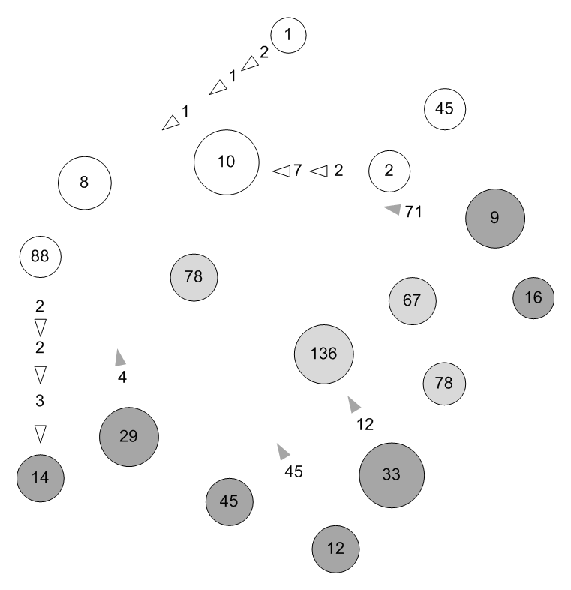
\includegraphics[scale=0.8]{imags/naves.eps}
%\end{center} 
%\caption{Example of execution of the Player Wars game. White planets and ships are owned by the player and dark gray ones are controlled by the enemy. Clear gray are neutral planets (not yet invaded).}
%\label{fig:naves}
%\end{figure}

In this work Genetic Programming (GP) is used to obtain agents that play 1 vs 1 battles in Planet Wars. The objective of GP is to create functions or programs to solve determined problems. Individual representation is usually in form of a tree, formed by operators (or {\em primitives}) and variables ({\em terminals}). These sets are usually fixed and known. The genome size is, therefore, variable, but the maximum size (depth) of the individuals is usually fixed, to avoid high evaluation costs. 

%GP has been used to evolve LISP (LISt Processing) programs \cite{Koza1990Tools}, or XSLT (eXtensible Stylesheet Language Transformations) scripts \cite{Garcia2008XSLT}, among others.

The aim of using GP in this scope is the creation of behavioural rule-based engines following an heuristic, algorithmic and automatic process. Thus, instead of implementing them from scratch by a human (expert or not), this method will define a set of rules that could be more complex (or simpler) than those defined by the humans. 

This work uses some of the results obtained in a previous one \cite{GPBot_EVO2014} as a baseline for comparisons. Three different fitness functions will be presented and tested here: the first one is our traditional \textit{turn-based fitness} \cite{Genebot_CEC11}, which evaluates all the individuals in the population by playing five different matches (in five different maps) against a sparring bot. The aim of the repetitions is to avoid the noisy factor present in this problems (videogames) \cite{Mora_noisy_jcst}. Due to which the fitness value for an individual could dramatically vary between different matches, since it depends on the pseudo-stochastic opponent's actions, and also on its own non-deterministic decisions.
The other two presented fitness functions also point to reduce the influence of noise in the evolution. Thus, they consider the number of ships generated by each bot rather than the number of turns and compute, respectively, a \textit{linear regression} based on the percentage of ships with respect to the total, and \textit{the integral} of the function which represents these numbers.
All of them consider the final results of every individual (bot) after the aforementioned five matches (on average).

The work is then focused on proving the value of these evolved rule-based control systems for the agents. To this end, several experiments have been conducted, considering the aforementioned fitness functions and some of our previous evolutionary bots as rivals in the comparisons.

%The rest of the work is structured as follows: after the state of the art, the description of our agent is presented in Section \ref{sec:agent}. Then, the experimental setup conduced with the GP is shown (Section \ref{sec:experiments}). Finally, results, conclusions and future works are discussed.
%
%*** Reescribir ***

%-----------------------------------------------------------------
%%%%%%%%%%%%%%%%%%%%%%%% BACKGROUND %%%%%%%%%%%%%%%%%%%%%%%%%%%%%%
%-----------------------------------------------------------------
\section{Background and problem description}

\subsection{Genetic Programming}

The Genetic Programming (GP) \cite{GP_Koza92} is a kind of Evolutionary Algorithm (EA) \cite{EAs_Back96} (a class of direct, probabilistic search and optimization algorithms gleaned from the model of darwinistic evolution), based on the idea that in nature structures undergo adaptation. It shares some common features with this algorithms: a population of possible solutions (individuals) of the target problem, a selection method that favours better solutions and a set of operators that act upon the selected solutions.
Thus, GP is a structural optimisation technique where the individuals are represented as hierarchical structures (typically tree structures) and the size and shape of the solutions are not defined a priori as in other methods from the field of evolutionary computation, but they evolve along the generations. So, the main difference with regard to GAs is the individual representation and the genetic operators to apply, which are mainly focused on the management (and improvement) of this kind of
structure.
The flow of a GP algorithm is the same as any other EA: a population is created at random, each individual in the population is evaluated using a fitness function, the individuals that performed better in the evaluation process have a higher probability of being selected as parents for the new population than the rest and a new population is created once the individuals are subjected to the genetic operators of crossover and mutation with a certain probability. The loop is run until a predefined termination criterion is met.

% ----------------------------------------------------------------------

\subsection{Planet Wars Game}

In this paper we work with a %simplified
version of the game Galcon, aimed at performing bot's fights which was used as base for the Google AI Challenge 2010 (GAIC)\footnote{http://ai-contest.com}.
% Maribel, a�ado el we que creo que faltaba no?

 \begin{figure}[ht]
 \begin{center}
   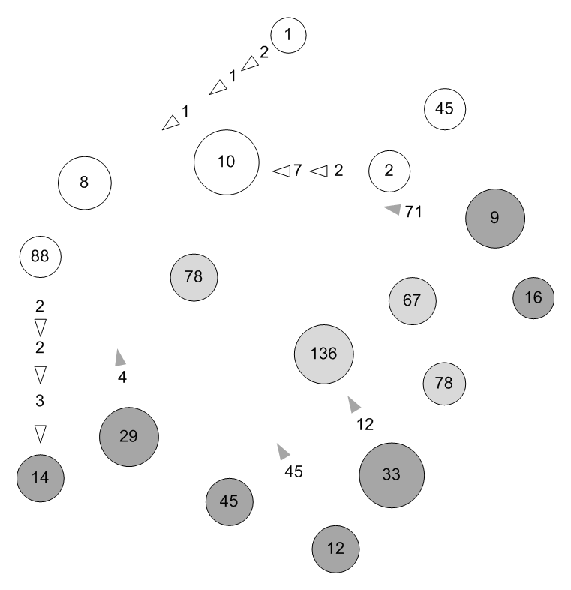
\epsfig{file=./imags/naves.eps,width=7cm}
 \end{center}
 \caption{Simulated screenshot of an early stage of a run in Planet Wars. White planets belong to the player (blue colour in the game), dark grey belong to the opponent (red in the game), and light grey planets belong to no player. The triangles are fleets, and the numbers (in planets and triangles) represent the ships. The planet size means growth rate of the amount of ships in it (the bigger, the higher).}
 \label{figura:PlanetWars1}
 \end{figure}

A Planet Wars match takes place on a map %(see Fig. \ref{figura:PlanetWars1}) 
that contains several planets (neutral, enemies or owned), each one of them with a number assigned to it that represents the quantity of ships that the planet is currently hosting. 

The aim of the game is to defeat all the ships in the opponent's planets. Although Planet Wars is a RTS game, this implementation has transformed it into a turn-based game, in which each player has a maximum number of turns to accomplish the objective. At the end of the match, the winner is the player that remains alive, or that which owns more ships if more than one survives. 

There are two strong constraints which determine the possible methods to apply to design a bot: a simulated turn takes \textit{just one second}, and the bot is \textit{not allowed to store any kind of information} about its former actions, about the opponent's actions or about the state of the game (i.e., the game's map).

Therefore, the aim in this paper is to study the improvement of a bot according to the state of the map in each simulated turn (input), returning a set of actions to perform in order to fight the enemy, conquering its resources, and, ultimately, wining the game. In the original game, only two bots are faced but in this paper it is studied what happen when we simulate 4 on 4 battles, i.e., when 4 bots are fighting in the same map.

%-----------------------------------------------------------------------
%%%%%%%%%%%%%%%%%%%%%%%% STATE OF THE ART %%%%%%%%%%%%%%%%%%%%%%%%%%%%%%
%-----------------------------------------------------------------------
\section{State of the art}
\label{sec:soa}

RTS games have been used extensively in the computational intelligence area (see \cite{Lara2013review} for a survey). 

Among other techniques, Evolutionary Algorithms (EAs) have been widely used as a  Computational Intelligence method in RTS games \cite{Lara2013review}. For example, for parameter optimization \cite{Esparcia10FPS}, learning \cite{Kenneth2005neuroevolution} or content generation \cite{Mahlmann2012MapGeneration}. 

One of these types, Genetic Programming, has been proved as a good tool for developing strategies in games, achieving results comparable to human, or human-based competitors \cite{Sipper2007gameplaying}. They also have obtained higher ranking than solvers produced by other techniques or even beating high-ranking humans \cite{Elyasaf2012FreeCell}. GP has also been used in different kind of games, such as board-games \cite{Benbassat2012Reversi}, or (in principle) simpler games such as Ms. Pac-Man \cite{Brandstetter2012PacMan} and Spoof \cite{Wittkamp2007spoof} and even in modern video-games such as First Person Shothers (FPS) (for example, Unreal\texttrademark~ \cite{Esparcia2013GPunreal}).
 
Planet Wars, the game used in this work, has also been used in other researches as an experimental framework for agent testing. 
We have deeply worked in this environment \cite{Genebot-IWANN2011,Genebot_CEC11,genebot-evo12,ExpGenebot_CIG2012,Co-Genebot_EVO2014}, mainly using Genetic Algorithms for evolving (the parameters of) a behavioural engine previously defined by a human expert from scratch. In those works we have proposed different implementations, analysed the noise influence, defined expert bots, or implemented co-evolutionary approaches.

%For example, in
%\cite{Mora2012Genebot} the authors programmed the behaviour of a {\em bot} (a computer-controlled player) with a decision tree of 3 levels. Then, the values of these rules were optimized using a genetic algorithm to tune the strategy rates and percentages.  
%  Results showed a good performance confronting with other bots
%  provided by the Google AI Challenge. %In our next work
%  In \cite{FernandezAres2012adaptive} the authors improved this agent optimizing it in different types of maps and selecting the set of optimized
%  parameters depending on the map where the game was taking place,
%  using a tree of 5 levels. These results outperformed the previous
%  version of the bot with 87\% of victories. 

In this paper we use GP to create the Decision Tree ***[REF]***, instead of expert human gaming experience to model it, and the resulting agent is compared with two bots previously presented: Genebot \cite{Genebot_CEC11}, our initial bot improved by means of Genetic Algorithms, and Exp-Genebot \cite{ExpGenebot_CIG2012} an enhanced agent which considers different sets of parameters depending on the type of battle map, which is previously analysed by the bot.


%-------------------------------------------------------------
%%%%%%%%%%%%%%%%%%%%%%%% GP BOT %%%%%%%%%%%%%%%%%%%%%%%%%%%%%%
%-------------------------------------------------------------
\section{GPBot}
\label{sec:agent}

The Genetic Programming-based bot or {\em GPBot} evolves a set of rules which, in turn, models a Decision Tree. During the evolution, every individual in the population (a tree) must be evaluated. To do so the tree is set as the behavioural engine of an agent, which is then placed in a map against a rival in a Planet Wars match. Depending on the obtained results the agent (i.e. the individual) gets a fitness value, that will be considered in the evolutionary process as a measure of its validity.
 
Thus, during the match the tree will be used (by the bot) in order to select the best strategy at every moment, i.e. for every planet a target will be selected along with the number of ships to send from one the other.

\noindent The used Decision Trees are binary trees of expressions composed by two different \textit{types of nodes}:

\begin{itemize}
\item {\em Decision}: a logical expression formed by a variable, a less than operator ($<$), and a number between 0 and 1. It is the equivalent to a ``primitive'' in the field of GP.
\item {\em Action}: a leave of the tree (therefore, a ``terminal''). Each decision is the name of the method to call from the planet that executes the tree. This method indicates to which planet send a percentage of available ships (from 0 to 1). 
\end{itemize}

\noindent The decisions are based in the values of different \textit{variables}, namely:

\begin{itemize}
\item {\em myShipsEnemyRatio}: Ratio between the player's ships and enemy's ships.
\item {\em myShipsLandedFlyingRatio}: Ratio between the player's landed and flying ships.
\item {\em myPlanetsEnemyRatio}: Ratio between the number of player's planets and the enemy's ones.
\item {\em myPlanetsTotalRatio}: Ratio between the number of player's planet and total planets (neutrals and enemy included).
\item {\em actualMyShipsRatio}: Ratio between the number of ships in the specific planet that evaluates the tree and player's total ships.
\item {\em actualLandedFlyingRatio}: Ratio between the number of ships landed and flying from the specific planet that evaluates the tree and player's total ships.
\end{itemize}

\noindent Finally, the possible \textit{decisions} are:

\begin{itemize}
\item {\em Attack Nearest (Neutral|Enemy|NotMy) Planet}: The objective is the nearest planet.
\item {\em Attack Weakest (Neutral|Enemy|NotMy) Planet}: The objective is the planet with less ships.
\item {\em Attack Wealthiest (Neutral|Enemy|NotMy) Planet}: The objective is the planet with higher lower rate.
\item {\em Attack Beneficial (Neutral|Enemy|NotMy) Planet}: The objective is the  more beneficial planet, that is, the one with highest growth rate divided by the number of ships.
\item {\em Attack Quickest (Neutral|Enemy|NotMy) Planet}: The objective is the planet easier to be conquered: the lowest product between the distance from the planet that executes the tree and the number of  ships in the objective planet.
\item {\em Attack (Neutral|Enemy|NotMy) Base}: The objective is the planet with more ships (that is, the base).
\item {\em  Attack Random Planet}.
\item {\em Reinforce Nearest Planet}: Reinforce the nearest player's planet to the planet that executes the tree.
\item {\em Reinforce Base}: Reinforce the player's planet with higher number of ships.
\item {\em Reinforce Wealthiest Planet}: Reinforce the player's planet with higher grown rate.
\item {\em Do nothing}.

\end{itemize}

\noindent An example of a possible decision tree is shown below. This example tree has a total of 5 nodes, with 2 decisions and 3 actions, and a depth of 3 levels.

\begin{verbatim}

if(myShipsLandedFlyingRatio < 0.796)
   if(actualMyShipsRatio < 0.201)
      attackWeakestNeutralPlanet(0.481);
   else
      attackNearestEnemyPlanet(0.913);
else
   attackNearestEnemyPlanet(0.819);

\end{verbatim}\\\\

\noindent The bot's behaviour is explained in Algorithm \ref{alg:turn}.

\begin{algorithm}[ht]
\begin{algorithmic}
%\SetAlgoLined
%\KwData{this text}
%\KwResult{how to write algorithm with \LaTeX2e }

\STATE // At the beginning of the execution the agent receives the tree
\STATE tree $\leftarrow$ readTree()
\WHILE{game not finished}
	\STATE // starts the turn
	\STATE calculateGlobalPlanets() // e.g. Base or Enemy Base
	\STATE calculateGlobalRatios() // e.g. myPlanetsEnemyRatio
	\FOR{Each p in PlayerPlanets}
		\STATE calculateLocalPlanets(p) // e.g. NearestNeutralPlanet to p
		\STATE calculateLocalRatios(p) //e.g actualMyShipsRatio
		\STATE executeTree(p,tree)  // Send a percentage of ships to destination
   \ENDFOR
\ENDWHILE

\end{algorithmic}
\caption{Pseudocode of the proposed agent. The same tree is used during all the agent's execution}
\label{alg:turn}
\end{algorithm}



%\COMMENT {In each turn}
%\LOOP
	
%	\STATE calculateGlobalPlanets()
%	\COMMENT{{\em for example Base, Enemy Base...}}
%	\STATE calculateGlobalRatios ()
%	\COMMENT {{\em for example myPlanetEnemyRatio, myShipsEnemyRatio...}}
%		\FOR{each Planet: p}
%			\STATE calculateLocalPlanets (p)
%			\COMMENT{{\em for example NearestNeutralPlanet to planet p}}
%			\STATE calculateLocalRatios (p)
%			\COMMENT{{\em for example actualMyShipsRatio}}
%			\STATE executeTree(p,tree)
%			\COMMENT{{\em Send a percentage of the ships to another planet}}
%		\ENDFOR
%\ENDLOOP

Next section is devoted to explain the main component of the evolutionary process, i.e. the fitness function. As previously stated, we have implemented three different functions, which are used to evaluate the agent's performance during the matches.

%-----------------------------------------------------------------------
%%%%%%%%%%%%%%%%%%%%%%%% FITNESS FUNCTIONS %%%%%%%%%%%%%%%%%%%%%%%%%%%%%
%-----------------------------------------------------------------------

\section{Fitness Functions}
\label{sec:fitness_functions}

*** ACLARAR ESTO con FERGU ***

In previous works *** [REF a trabajos de Genebot] ***, a bot was evaluated always versus the same enemy (a reference bot), several times (in different maps). The fitness function was defined depending on the result of the battle (if the bot wins all its battles or loses in any of them) and the number of turns needed for ending the game. 
For two bots, A and B the fitness was defined as Algorithm \ref{alg:fitness_turns_positions} shows.

\begin{algorithm}[ht]
\begin{algorithmic}
        
\STATE $A,B \in Population$
\IF{A WINs always}
	\IF{B LOSEs some battle}
		\STATE A is better than B
	\ELSE
		\IF{A take less turns than B}
			\STATE A is better than B
      \ELSE
			\STATE B is better than A
      \ENDIF
	\ENDIF   
\ELSE
	\IF{B WINs always}
		\STATE B is better than A
	\ELSE
		\IF{A take less turns than B}
			\STATE B is better than A
		\ELSE
			\STATE A is better than B
		\ENDIF
	\ENDIF
\ENDIF

\end{algorithmic}
\caption{Fitness function based in turns and positions}
\label{alg:fitness_turns_positions}
\end{algorithm}

In this fitness, we are only interested in the final result (position and number of turns). We do not include in the analysis how the bot has reached them. The problem of this function is that the consideration of two different terms makes it difficult the comparison between different evaluations. 

This fitness works well for 1 vs 1 battles, it has some limitations *** PROBLEMAS DEL FITNESS ***  that should be addressed. In this work two additional evaluation functions have been proposed in order to let easier and fairer comparison methods between bots. *** intenta paliar en cierta medida el ruido [REF al ruido] ***

Both of them are based in the percentage of ships belonging to each player in every turn. They are normalized considering the total number of ships in the game for that turn (including neutrals ships in neutral planets). For each player, we have a different {$cloud$} of ships as Fig.\ref{figura:nubecita} shows. 

\begin{figure}[ht]
\begin{center}
  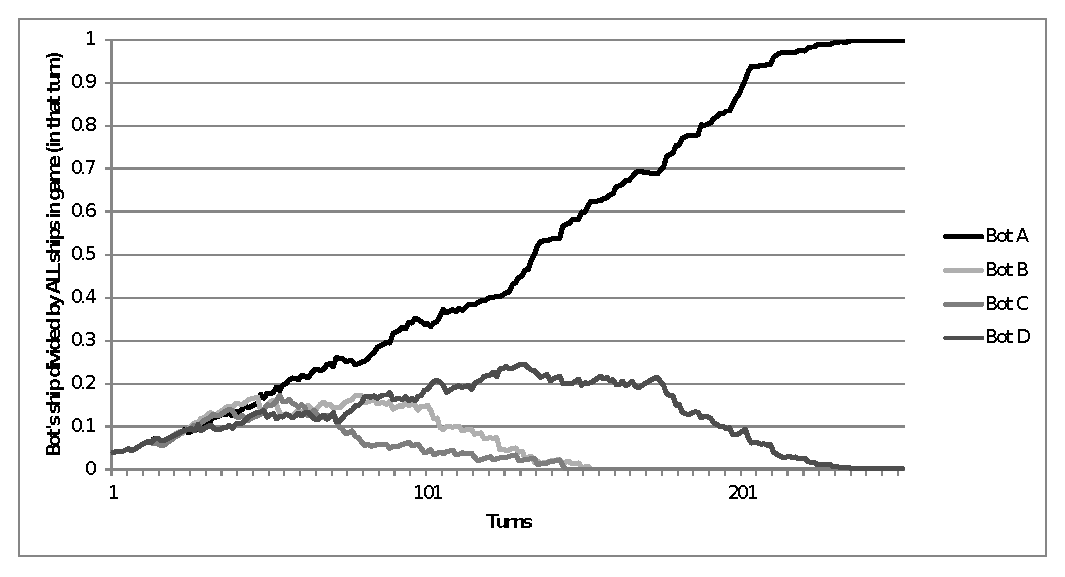
\epsfig{file=imags/nubecita.eps,width=6cm}
\end{center}
\caption{Representation of the number of ships of each bot in each turn} 
\label{figura:nubecita}
\end{figure}

Below, are described the two alternatives to deal with this cloud of points for the fitness function: the use of slopes and areas.

% ---------------------------------------------------------------------

\subsection{Fitness based in Slope.}
\label{subsec:fitness_slope}

For this fitness, a square regression analysis is computed in order to transform the cloud of points into a simple line. The line is represented as {$y = \alpha \times x + \beta $}, where {$\alpha$} and {$\beta$} are calculated as shown in Equations \ref{eq:alpha} and \ref{eq:beta}, computing a least squares regression. For every bot in the simulation we calculate $\alpha$ and ($slope$). This $slope$ is the fitness of every bot for that simulation. 

%A graphical example can be seen in Fig. \ref{figura:nubecita:pendiente}.

%%Antonio, pon esto junto si puedes, en la misma fila, que con subfigure no funciona :(
\begin{equation}
\label{eq:alpha}
        \alpha = \frac{\sum_{i=1}^{n}(X_{i} - \bar{X_{i}})(Y_{i} - \bar{Y_{i}})}{\sum_{i=1}^{n}(X_{i} - \bar{X_{i}})^{2}}
\end{equation}

\begin{equation}
\label{eq:beta}
        \beta = \bar{Y}-\alpha\bar{X}
\end{equation}


%\begin{figure}[h]
%\centering
%\hspace*{-1in}
%  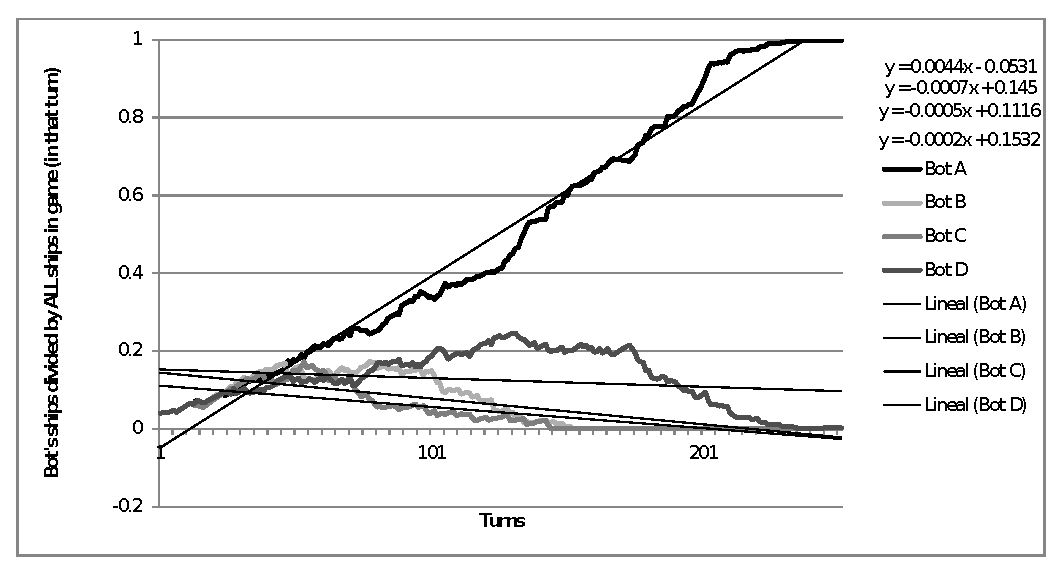
\epsfig{file=imagenes/nubecita_pendiente.eps,width=0.6
%  \textwidth}
%\caption{Fitness based in Slope: number of ships of every bot in each turn}
%\label{figura:nubecita:pendiente}
%\end{figure}


%\begin{figure}[h]
%\centering
%\hspace*{-1in}
%\begin{subfigure}[H]{0.4\textwidth}
%	\large
%    \begin{equation}
%        \alpha = \frac{\sum_{i=1}^{n}(X_{i} - \bar{X_{i}})(Y_{i} - \bar{Y_{i}})}{\sum_{i=1}^{n}(X_{i} - \bar{X_{i}})^{2}}
%    \end{equation}
%    \begin{equation}
%        \beta = \bar{Y}-\alpha\bar{X}
%    \end{equation}
%    \caption{Least Squares Regression}
%    \label{equation:LeastSquares}
%\end{subfigure}
%\hfill
%\hspace*{0.2in}
%\begin{subfigure}[H]{0.7\textwidth}
%\begin{center}
%  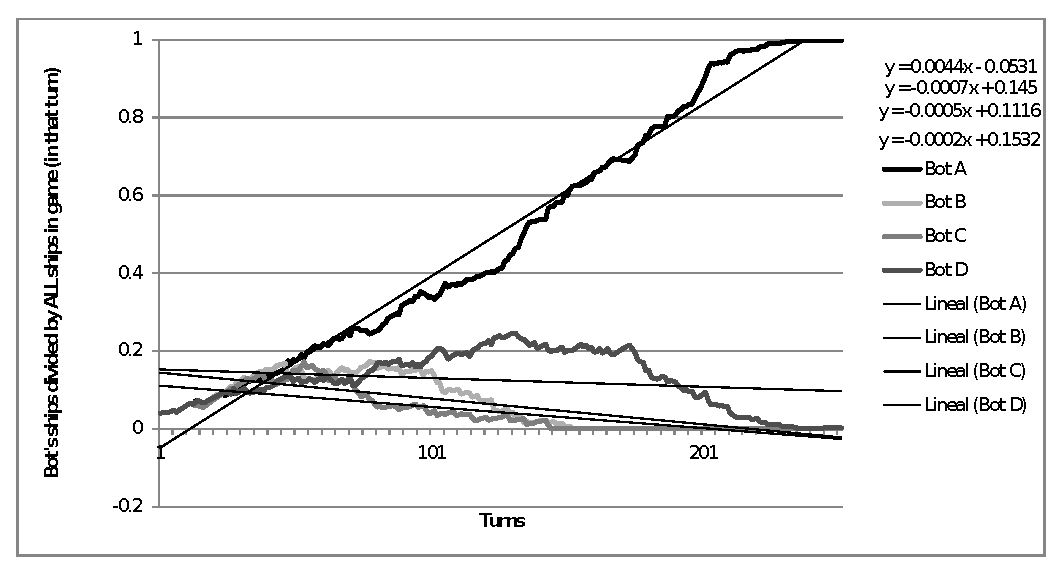
\epsfig{file=imagenes/nubecita_pendiente.eps,width=1.1\textwidth}
%\end{center}
%\caption{Number of ships of every bot in each turn} %Maribel, cambio if por of
%\label{figura:nubecita:pendiente}
%\end{subfigure}
%\caption{Fitness based in Slope}
%\end{figure}

Theoretical maximum and minimum values are set for this fitness. An optimum bot that wins in the first turn, has an ideal slope of {$1$}, so this is the maximum value of our fitness. On the other hand, a bot that loses in the first turn,  has a slope of {$-1$}. Thus, if we calculate the $slope$, we know if the bot {$WINs$} ({$slope>0$}) or {$LOSEs$} {$slope<0$}. 
The values of the different battles are summed to compute the global $slope$. Then, the bot with the highest value will be the best is each turn or battle. 

%Several evaluations in different maps was using, so it's need operate with fitness. In that case, only sum the slope of all the evaluations of the bot. Maribel, esto ya lo has dicho antes y adem�s l�a m�s la cosa as� que lo he eliminado. Adem�s expresiones como "was using" est�n mal, qu� quieres decir? fue usando? eso en ingl�s no se dice.

% ---------------------------------------------------------------------

\subsection{Fitness based in Area.}
\label{sec:fitness}

In this case, the integral of the curve of the bot's live-line is used for calculating the area that is `covered' by the fitness cloud of points (see Equation \ref{eq:area}). This {$area$} is normalized considering the number of turns, and thus it represents the average percentage of ships during the battle for each player. 
%An example is shown in Fig. \ref{figura:nubecita:area}.

\begin{equation}
        area=\frac{\int_{0}^{t}\%ships(x)dx}{t}
    \label{eq:area}
\end{equation}

% \begin{figure}[h]
% \begin{center}
%   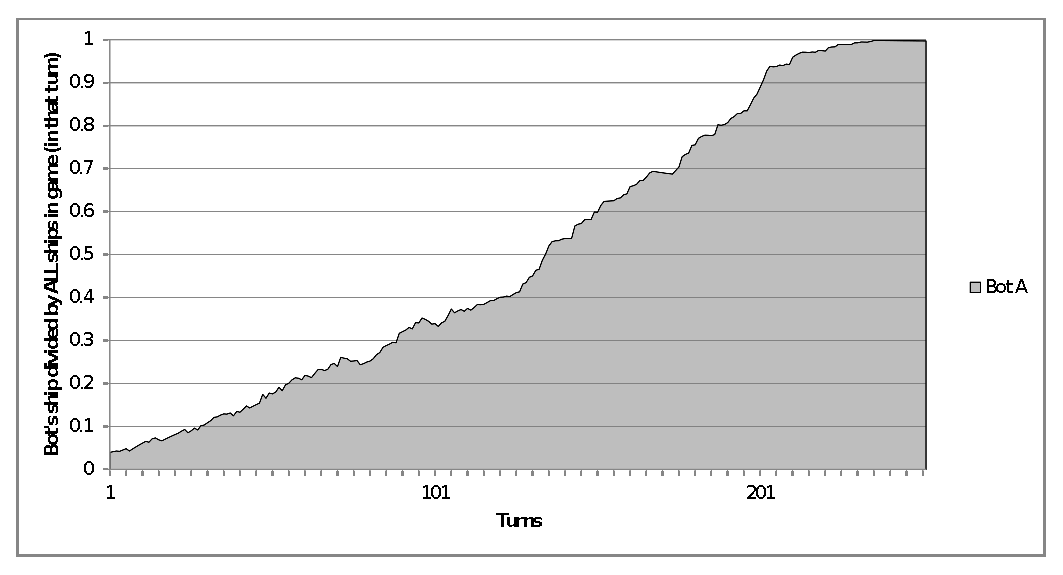
\epsfig{file=imagenes/nubecita_integral.eps,width=0.7\textwidth}
% \end{center}
% \caption{Fitness based in Area. Example of area under the live-line curve.}
% \label{figura:nubecita:area}
% \end{figure}

%\begin{figure}[h]
%\centering
%\hspace*{-1in}
%\begin{subfigure}[H]{0.4\textwidth}
%	\large
%    \begin{equation}
%        area=\frac{\int_{0}^{t}\%ships(x)dx}{t}
%    \end{equation}
%    \caption{Calculus of the area}
%    \label{equation:area}
%\end{subfigure}
%\begin{subfigure}[H]{0.6\textwidth}
%\begin{center}
%  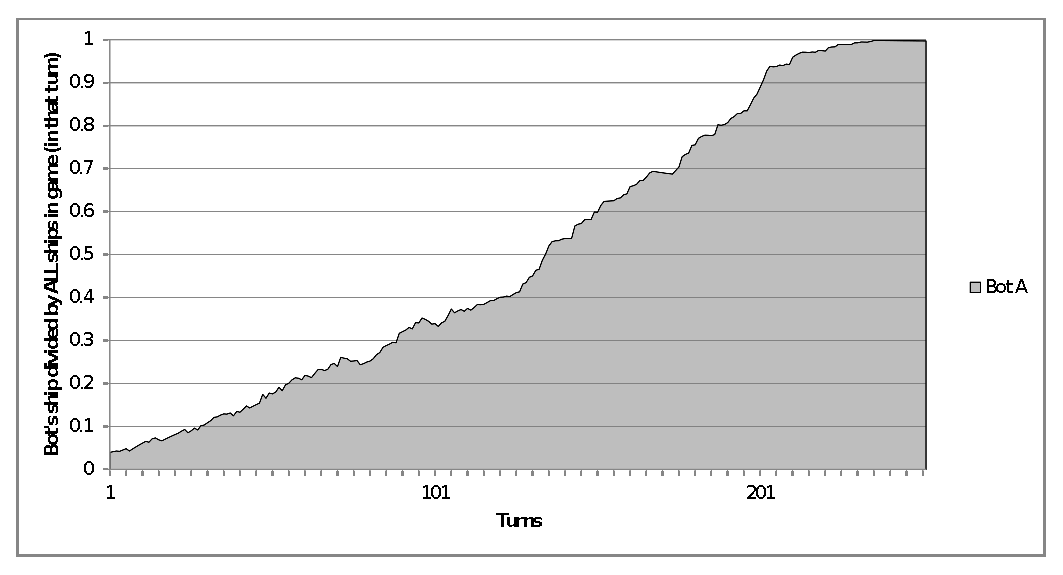
\epsfig{file=imagenes/nubecita_integral.eps,width=0.6\textwidth}
%\end{center}
%\caption{Example of area under the live-line curve.} 
%\label{figura:nubecita:area}
%\end{subfigure}
%\caption{Fitness based in Area}
%\end{figure}

As in previous case, maximum and minimum values has been set for this fitness. If an optimal bot wins in the first turn, the area of each live-line is close to {$1$}, so this is the maximum value of the fitness. Otherwise, if a bot loses in the first turn, its live-line area is close to {$0$}. In this case, we do not extract additional about which bot wins the battle, because the area of the live-line is not related with the winner of the battle. Thus, we are losing some information.

%-----------------------------------------------------------------------
%%%%%%%%%%%%%%%%%%%%%%%% EXPERIMENTAL SETUP %%%%%%%%%%%%%%%%%%%%%%%%%%%%
%-----------------------------------------------------------------------

\section{Experimental Setup}
\label{sec:experiments}

Sub-tree crossover and 1-node mutation evolutionary operators have been used, following other researchers' proposals that have used these operators obtaining good results \cite{Esparcia2013GPunreal}. In this case, the mutation randomly changes the decision of a node or mutate the value with a step-size of 0.25 (an adequate value empirically tested). Each configuration is executed 30 times, with a population of 32 individuals and a 2-tournament selector for a pool of 16 parents.

To test each individual during the evolution, a battle with a previously created bot is performed in 5 different (but representative) maps provided by Google is played. Hierarchical fitness is used, as proposed in \cite{Genebot_CEC11}. Thus, an individual is better than another if it wins in a higher number of maps. In case of equality of victories, then the individual with more turns to be defeated (i.e. the stronger one) is considered better. The maximum fitness is, therefore 5 victories and 0 turns. Also, as proposed by \cite{Genebot_CEC11}, and due to the noisy fitness effect, all individuals are re-evaluated in every generation.


Two publicly available bots have been chosen for our experiments\footnote{Both can be downloaded from \url{https://github.com/deantares/genebot}}. The first bot to confront is {\em GeneBot}, proposed in \cite{Genebot_CEC11}. This bot was trained using a GA to optimize the 8 parameters that conforms a set of hand-made rules, obtained from an expert human player experience. The second one is an advanced version of the previous, called {\em Exp-Genebot} (Expert Genebot) \cite{}. This bot outperformed Genebot widely. Exp-Genebot bot analyses the distribution of the planets in the map to chose a previously optimized set of parameters by a GA.  Both bots are the best individual obtained of all runs of their algorithm (not an average one).

After running the proposed algorithm without tree limitation in depth, it has also been executed with the lower and average levels obtained for the best individuals: 3 and 7, respectively, to study if this number has any effect on the results.   Table \ref{tab:parameters} summarizes all the parameters used.

\begin{table}
\begin{center}
\begin{tabular}{|c|c|}
\hline
{\em Parameter Name} & {\em Value} \\\hline
Population size & 32 \\\hline
Crossover type & Sub-tree crossover \\ \hline
Crossover rate & 0.5\\ \hline
Mutation  & 1-node mutation\\ \hline
Mutation step-size & 0.25 \\ \hline
Selection & 2-tournament \\ \hline
Replacement & Steady-state\\ \hline
Stop criterion & 50 generations \\ \hline
Maximum Tree Depth & 3, 7 and unlimited \\ \hline
Runs per configuration & 30 \\ \hline
Evaluation & Playing versus Genebot \cite{Genebot_CEC11} and Exp-Genebot \cite{ExpGenebot_CIG2012} \\ \hline
Maps used in each evaluation & map76.txt map69.txt map7.txt map11.txt map26.txt \\ \hline
\end{tabular}
\caption{Parameters used in the experiments.}
\label{tab:parameters}
\end{center}
\end{table}

After all the executions we have evaluated the obtained best individuals in all runs confronting to the bots in a larger set of maps (the 100 maps provided by Google) to study the behaviour of the algorithm and how good are the obtained bots in maps that have not been used for training.

The used framework is OSGiLiath, a service-oriented evolutionary framework \cite{Garcia13Service}. The generated tree is compiled in real-time and injected in the agent's code using Javassist \footnote{\url{www.javassist.org}} library. All the source code used in this work is available under a LGPL V3 License in \url{http://www.osgiliath.org}.


%-------------------------------------------------------------
%%%%%%%%%%%%%%%%%%%%%%%% RESULTS %%%%%%%%%%%%%%%%%%%%%%%%%%%%%
%-------------------------------------------------------------
\section{Results}

Tables \ref{tab:resultsGenebot} and \ref{tab:resultsExpgenebot} summarize all the obtained results of the execution of our EA. These tables also show the average age, depth and number of nodes of the best individuals obtained and also the average population at the end of the run. The average turns rows are calculated only taking into account the individuals with a number of victories lower than 5, because this number is 0 if they have won the five battles.



\begin{table*}
\centering{
\begin{tabular}{|c|c|c|c|c|} \hline
    \multicolumn{2}{|c|}{}    &  {\em Depth 3}                & {\em Depth 7}                &    {\em Unlimited  Depth}    \\ \hline  
\multirow{2}{*}{Best Fitness}  & Victories     &   \textbf{4.933} $\pm$ 0.25       &  4.83 $\pm$ 0.53       &    4.9     $\pm$ 0.30  \\ \cline{2-5}  
              & Turns         &  244.5 $\pm$  54.44     &  466   $\pm$ 205.44    &    266.667 $\pm$ 40.42 \\ \hline  
\multirow{2}{*}{Population Ave. Fitness}  & Victories     &   \textbf{4.486}$\pm$ 0.52 & 4.43 $\pm$ 0.07   &    4.711   $\pm$ 0.45  \\ \cline{2-5}  
              & Turns         &  130.77$\pm$ 95.81      &  139.43 $\pm$ 196.60   &    190.346 $\pm$ 102.92\\ \hline  
\multirow{2}{*}{Depth}         & Best          &  3     $\pm$ 0          & 5.2 $\pm$ 1.78         &    6.933   $\pm$ 4.05  \\ \cline{2-5}
              & Population    &  3  $\pm$ 0             & 5.267 $\pm$ 1.8        &    7.353   $\pm$ 3.11  \\ \hline  
\multirow{2}{*}{Nodes}         & Best          &  7     $\pm$ 0          &   13.667 $\pm$ 7.68    &    22.133  $\pm$ 22.21 \\ \cline{2-5}  
              & Population    &  7     $\pm$ 0          & 13.818 $\pm$ 5.86      &    21.418  $\pm$ 13.81 \\ \hline  
\multirow{2}{*}{Age}           & Best          &  \textbf{8.133} $\pm$ 3.95       & 5.467 $\pm$ 2.95       &    5.066   $\pm$ 2.11  \\ \cline{2-5}
              & Population    &  \textbf{4.297} $\pm$ 3.027      & 3.247 $\pm$ 0.25       &    3.092   $\pm$ 1.27  \\ \hline
\end{tabular}
\caption{Average results obtained from each configuration versus Genebot. Each one has been tested 30 times.}
\label{tab:resultsGenebot}
}
\end{table*}

\begin{table*}
\centering{
\begin{tabular}{|c|c|c|c|c|} \hline            
 \multicolumn{2}{|c|}{}        &  {\em Depth 3}                & {\em Depth     7}            &   {\em Unlimited Depth}     \\ \hline  
\multirow{2}{*}{Best Fitness}  & Victories     &   4.133   $\pm$ 0.50    & 4.2      $\pm$ 0.48    &   \textbf{4.4}     $\pm$ 0.56  \\ \cline{2-5} 
              & Turns          &  221.625 $\pm$ 54.43   & 163.667  $\pm$ 106.38  &   123.533 $\pm$ 112.79\\ \hline 
\multirow{2}{*}{Population Ave. Fitness}  & Victories      &  3.541   $\pm$ 0.34    & 3.689    $\pm$ 0.37    &   \textbf{4.043}   $\pm$ 0.38  \\ \cline{2-5} 
              & Turns          &  200.086 $\pm$ 50.79   & 184.076  $\pm$ 57.02   &   159.094 $\pm$ 61.84 \\ \hline  
\multirow{2}{*}{Depth}         & Best           &  3       $\pm$ 0       & 5.2      $\pm$ 1.84    &   6.966   $\pm$ 4.44  \\ \cline{2-5} 
              & Population     &  3       $\pm$ 0       & 5.216    $\pm$ 0.92    &   6.522   $\pm$ 1.91  \\ \hline 
\multirow{2}{*}{Nodes}         & Best           &  7       $\pm$ 0       & 12.6     $\pm$ 6.44    &   18.466  $\pm$ 15.46 \\ \cline{2-5}   
              & Population     &  7       $\pm$ 0       & 13.05    $\pm$ 3.92    &   16.337  $\pm$ 7.67  \\ \hline 
\multirow{2}{*}{Age}           & Best           &  4.266   $\pm$ 5.01    & 4.133    $\pm$ 4.26    &   \textbf{4.7}     $\pm$ 4.72  \\ \cline{2-5} 
              & Population     &  3.706   $\pm$ 0.58    & 3.727    $\pm$ 0.62    &   \textbf{3.889}   $\pm$ 0.71  \\ \hline  


\end{tabular}
\caption{Average results obtained from each configuration versus Exp-Genebot. Each one has been tested 30 times.}
\label{tab:resultsExpgenebot}
}
\end{table*}

As can be seen, the average population fitness versus Genebot is nearest to the optimum than versus Exp-Genebot, even with the lowest depth. Highest performance in the population is also with the depth of 3 levels. On the contrary, confronting with Exp-Genebot the configuration with unlimited depth achieves better results. This make sense as more decisions should be taken because the enemy can be different in each map.

In the second experiment, we have confronted the 30 bots obtained in each configuration again with Genebot and Exp-Genebot, but in the 100 maps provided by Google. This experiment has been used to validate if the obtained individuals of the proposed method can be competitive in terms of quality in maps not used for evaluation. Results are shown in Table \ref{tab:allmaps} and boxplots in Figure \ref{fig:victories}. It can be seen that in average, the bots produced by the proposed algorithm perform equal or better than the best obtained by the previous authors. Note that, even obtaining individuals with maximum fitness (5 victories) that have been kept in the population several generations (as presented before in Tables \ref{tab:resultsGenebot} and \ref{tab:resultsExpgenebot}) cannot be representative of a extremely good bot in a wider set of maps that have not been used for training. As the distributions are not normalized, a Kruskal-Wallis test has been used, obtaining significant differences in turns for the experiment versus Genebot (p-value = 0.0028) and victories in Exp-genebot (p-value = 0.02681). Therefore, there are differences using a maximum depth in the generation of bots. In both configurations, the trees created with 7 levels of depth as maximum have obtained the better results.

To explain why results versus Genebot (a weaker bot than Exp-Genebot) are slightly worse than versus Exp-Genebot, even when the best individuals produced by the GP have higher fitness, it is necessary to analyse how the best individual and the population are being evolved. Figure \ref{fig:gens} shows that best individual using Genebot reaches the optimal before Exp-Genebot, and also the average population converges quicker. This could lead to over-specialization: the generated bots are over-trained to win in the five maps. This is due because these individuals are being re-evaluated, and therefore, they are still changing after they have reached the optimal.



\begin{table*}
\centering{
\begin{tabular}{|c|c|c|c|c|c|c|} \hline
   
    
  


{\em Configuration}     &    {\em Average maps won}  &    {\em Average turns}     \\ \hline
                   \multicolumn{3}{|c|}{Versus Genebot}    \\ \hline
 Depth 3          &   47.033 $\pm$ 10.001 &   133.371 $\pm$   16.34    \\ \hline
 Depth 7          &   48.9 $\pm$ 10.21    &   \textbf{141.386} $\pm$  15.54   \\ \hline
 Unlimited Depth  &   50.23 $\pm$ 11.40   &   133.916   $\pm$   10.55    \\ \hline
       \multicolumn{3}{|c|}{Versus Exp-Genebot}                          \\ \hline              
 Depth 3          &   52.367 $\pm$ 13.39 &  191.051 $\pm$ 67.79 \\ \hline
 Depth 7          &   \textbf{58.867} $\pm$ 7.35  &  174.694$\pm$ 47.50 \\ \hline
 Unlimited Depth  &   52.3 $\pm$ 11.57   &  197.492 $\pm$ 72.30 \\ \hline 

\end{tabular}


\caption{Results confronting the 30 best bots attained from each configuration in the 100 maps each.}
\label{tab:allmaps}
}
\end{table*}

\begin{figure}[htb]
\centering

\subfigure[Victories]{
   \includegraphics[scale =0.30] {imags/victories.eps}
   \label{fig:subfig1}
 }
\subfigure[Turns]{
   \includegraphics[scale =0.30] {imags/turns.eps}
   \label{fig:subfig2}
 }
\caption{Average of executing the 30 best bots in each configuration (3, 7 and U) versus Genebot (G) and Exp-Genebot (E).}

\label{fig:victories}
\end{figure}

\begin{figure}[htb]
\centering
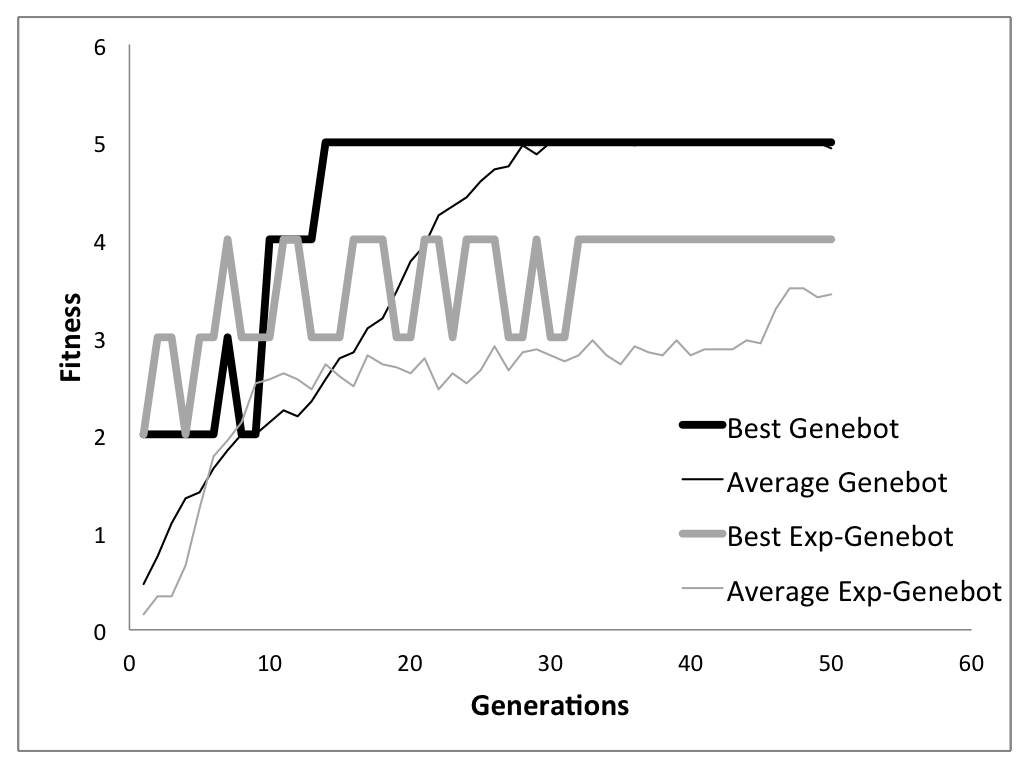
\includegraphics[scale =0.60] {imags/generations.eps}
\caption{Evolution of the best individual and the average population during one run for depth 7 versus Genebot and Exp-Genebot.}
\label{fig:gens}
\end{figure}


%-----------------------------------------------------------------
%%%%%%%%%%%%%%%%%%%%%%%% CONCLUSIONS %%%%%%%%%%%%%%%%%%%%%%%%%%%%%
%----------------------------------------------------------------- 
\section{Conclusions}
\label{sec:conclusion}

This work presents a Genetic Programming algorithm that generates agents for playing the Planet Wars game. A number of possible actions to perform and decision variables have been presented. Two competitive bots available in the literature (Genebot and Exp-Genebot) have been used to calculate the fitness of the generated individuals. These two bots were the best obtained from several runs and the behaviour to be optimized was extracted from human expertise. Three different maximum depth for the trees have been used: 3, 7 and unlimited. Results show that the best individuals outperform these agents during the evolution in all configurations. These individuals have been tested against a larger set of maps not previously used during the evolution, obtaining equivalent or better results than Genebot and Exp-Genebot.

In future work, other rules will be added to the proposed algorithm (for example, the ones that analyse the map, as the Exp-Genebot does) and different enemies will be used. Other games used in the area of computational intelligence in videogames, such as Unreal\texttrademark~ or Super Mario\texttrademark~ will be tested.

\section*{Acknowledgements}
This work has been supported in part by FPU research grant AP2009-2942 and projects SIPESCA (G-GI3000/IDIF, under Programa Operativo FEDER de Andaluc�a 2007-2013), EvOrq (TIC-3903), CANUBE (CEI2013-P-14), ANYSELF (TIN2011-28627-C04-02) and PYR-2014-17 included in GENIL - CEI BIOTIC (Granada).

\bibliographystyle{splncs}
\bibliography{gpbot,genebot}



\end{document}

